\documentclass[a4paper, conference]{ieeeconf}
\usepackage{graphicx}

\title{
  \LARGE \bf Resumes Named Entity Recognition with Conditional Random Fields
}
\author{%
  Juan Alejandro Alcántara Minaya\\ \email{A01703947@exatec.tec.mx}
  \and
  Dr. Benjamín Valdés Aguirre\\ \email{bvaldes@tec.mx}
}

\begin{document}

  \maketitle
  \begin{abstract}
    We propose Lorem ipsum dolor sit amet, consecteuer
  \end{abstract} 

  \tableofcontents

  \section{Introduction}

  \section{Literature Review}
  \subsection{Named Entity Recognition (NER)}
  Named Entity Recognition is a subarea of Natural Language Processing. Its
  objective is to locate and categorize important words in a text. This process
  is crucial in applications that focus on information extraction, translation,
  and overall text analysis. Usually, named entities are classified according
  to the information they provide. For example, NER tasks frequently focus on
  extracting people, locations, and organizations from large text corpora
  \cite{Mohit2014}.

  There are two main challenges in named entity recognition tasks. The first
  one is determining the correct boundaries for a certain entity and the second
  one is determining the correct class for said entity. The author explains
  that there are ambiguous examples where it is easy for the models to make a
  mistake. For instance, the word \textit{Fox} can be interpreted as either a
  person or an organization. Another challenge arises when you consider that
  different domains consider different entities essential. For example, in
  resumes, the word \textit{Python} can refer to a skill, whereas in biology it
  may be referring to an animal. It is, therefore, crucial to have specifically
  labeled corpora tailored for the specific domain. \cite{Mohit2014}

  \subsection{Conditional Random Fields (CRF)}
  Conditional Random Fields are undirected probabilistic graphical models
  that tackle sequence analysis. It is often confused with Hidden Markov Models
  (HMMs) since they share some similarities. However, the main difference is
  that HMMs are a form of generative model and to "define a joint
  distribution... [it] must enumerate all possible observation sequences
  - a task which... is intractable unless observation elements are
  represented as isolated units" \cite{Wallach2004}.

  Nonetheless, Conditional Random Fields can model the dependency between
  different observations without having to increase model complexity. This
  property also allows the model to consider past and future tokens for the
  probabilistic prediction of the current token \cite{Lafferty2001}.
  \begin{figure}[h]
    \centering
    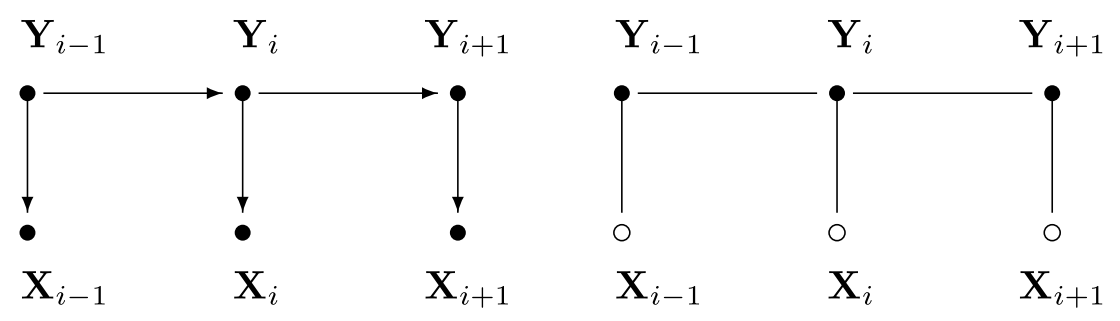
\includegraphics[width=\columnwidth]{hmm_vs_crf.png}
    \caption{%
      Graphical structures of simple HMMs (left), and chain-structured case of
      CRFs (right) for sequences. An open circle indicates that the variable is
      not generated by the model. \cite{Lafferty2001}
    }
  \end{figure}

  Most

  \section{Related Work} Resumes fall into the category of semi-structured
  documents. This characteristic poses a challenge for traditional parsing
  methods because the contents, although usually grouped by topic, do not share
  a single format. Computer scientists have had to rely on natural language
  processing (NLP) techniques to extract the relevant content. Different
  authors have used part of speech (POS) tagging, \textit{stop word} removal,
  and stemming to process the resume text content
  \cite{Sanyal2015,Ayishathahira2018a,Roy2020a}.

  \subsection{English Resume Parsing}
  Roy et al. \cite{Roy2020a} performed another survey of different classifier
  models such as Random Forests, Multinomial Naive Bayes, Logistic Regression,
  and Linear Support Vector Machines (LSVM). Their objective was to classify
  resumes into different job sectors such as sales, consulting, finance,
  technology, etc. To feed the data into the models they had to remove junk
  characters, and \textit{stop words} from the resumes. They also had to use
  stemming and lemmatization. This led to data loss, which is mentioned in the
  limitations. However, their objective was not to gather the specifics of
  their resumes, but instead to get a general idea of the candidate profile.
  Their research showed that the most performant model was the LSVM, with an
  average accuracy of 78.53\%.

  This survey showcases that for resume parsing the best model is usually the
  model that excels at sequence analysis. It shouldn't come as a surprise since
  resumes are semi-structured documents.

  \medskip
  On this note, Ayishathahira et al. \cite{Ayishathahira2018a} focused on
  effectively gathering named entities by comparing the performance of four
  models:
  \begin{itemize}
    \item Convolutional Neural Network (CNN)
    \item Bidirectional Long Short-Term Memory (Bi-LSTM)
    \item Conditional Random Field (CRF)
    \item Bi-LSTM and CNN combination (Bi-LSTM-CNN)
  \end{itemize}
  They worked with a dataset of 800 resumes sourced privately by one of their
  sponsors. They removed punctuations and other extraneous characters as well.
  Nevertheless, the authors didn't use lemmatization or stemming which allowed
  the sequences to remain mostly intact.

  Ayishathahira et. al defined 23 labels to classify information about a
  candidate's education, occupation, and identification. They trained the
  models to discover that the CRF implementation yielded the best results. On
  average, the CRF model had an F-score of 83.70\% while the Bi-LSTM-CNN had an
  F-score of 68.43\%. The CRF model beat the Bi-LSTM-CNN model across all the
  labels, with an average improvement of 15.26\%.

  The CRF model showed great advantages over its counterparts. It is relatively
  fast to train, needing less than half an hour to go through the authors'
  dataset. This speed, combined with its accuracy, makes the CRF model a great
  candidate to develop effective resume parsing tools.

  \medskip
  E. Suhas and E. Manjunath \cite{E*2020} took Ayishathahira's
  \cite{Ayishathahira2018a} research even further and they were able to develop
  a mixed model that allowed them to match candidates with job postings. The
  model is a combination of Named Entity Recognition (NER) and Word2Vec
  embedding to find the cosine distance between entities in resumes and job
  postings.

  They generated four different iterations of the NER model using, Stanford's
  NER model as a basis. They either removed more noise or increased the dataset
  size on each iteration and this translated to an F-score increase from about
  52\% to more than 80\%. The largest increase, of about 15\%, was achieved
  from the third iteration to the fourth iteration by introducing a dictionary
  of technical skills to the NER and increasing the window size.

  Even though this study had a smaller dataset than Ayishathahira's
  \cite{Ayishathahira2018a}, they were able to achieve similar results. Since
  it is a time-consuming and arduous process to prepare these datasets, this
  strategy is a great alternative to get the most out of the available
  resources.

  \subsection{Spanish Named Entity Recognition}
  Based on the research done for English corpus, Copara et. al
  \cite{Copara2016} developed a model that allowed named entity recognition for
  Spanish text. They decided to evaluate their model by using the CoNLL-2002
  (Spanish) dataset since it allows them to compare their performance against
  the state of the art.

  The authors decided to use word embedding and clustering in hopes of
  achieving better results. They used a large corpus of text both in Spanish
  and English to generate robust embeddings. Their baseline model achieved an
  F-Score of 80.02\%. After adding embedding and clustering, they were able to
  increase this score to 82.30\%. They noticed that there are words that are
  more likely to belong to one class than to another class and decided to use
  distributional prototypes to leverage this pattern. After adding prototypes,
  the model's F-Score dropped to 81.19\%. Nevertheless, they had the hypothesis
  that some entities share very similar features across languages and decided
  to use the Brown clusters from English. The model's F-score increased to
  82.44\%.

  Although the study didn't cover resumes specifically, it showcased various
  strategies to get better performance, even with a Spanish dataset. The most
  impressive observation is that the CRF model performed very similarly to the
  current state-of-the-art Deep Learning models.

  \section{Problem Statement} According to the Economic Commission for Latin
  America and the Caribbean (ECLAC), in 2019, an estimated average of 3.8
  million workers searched for work daily \cite{Hilbert2020a}. The same report
  estimated a daily average of 1.4 million job offer calls \cite{Hilbert2020a}.
  The supply is almost three times the demand, and it presents itself as an
  unmanageable task for recruiters across the region. Finding the best employee
  for a position is time-consuming since it requires combing through many
  candidates, and often missing essential information.

  \medskip
  The problem is that while in English-speaking countries there are tools to
  aid companies to handle the sheer volume of applications, there is not enough
  research to create these tools for Spanish-speaking countries.

  \section{Solution}
  \section{Evaluation}
  \section{Results}
  \section{Conclusions}
  \section{Future Work}
  \begin{itemize}
    \item Unsupervised CRF features
  \end{itemize}
  \subsection{Text Embedding}

  \bibliographystyle{ieeetr} \bibliography{library}

\end{document}
